\documentclass[11pt]{scrartcl}
\usepackage{polski}
\usepackage[polish]{babel}

\usepackage{graphicx, float, caption, subcaption, amsmath}
\usepackage{tabularx, multirow, hyperref, enumitem, listings}
%\usepackage{minted}

\usepackage{listings, xcolor}
\definecolor{md-black}{rgb}{0.12, 0.12, 0.12}
\definecolor{md-teal}{rgb}{0.38, 0.79, 0.69}
\definecolor{md-mauve}{rgb}{0.76, 0.52, 0.75}
\definecolor{md-green}{rgb}{0.13, 0.55, 0.13}
\definecolor{md-red}{rgb}{0.82, 0.10, 0.14}
\definecolor{md-purple}{rgb}{0.69, 0.33, 0.73}
\definecolor{md-orange}{rgb}{0.96, 0.42, 0.18}
\definecolor{md-gray}{rgb}{0.44, 0.46, 0.51}

\lstset{
    language=Python,
    basicstyle=\color{md-teal}\ttfamily,
    keywordstyle=\color{md-mauve},
    commentstyle=\color{md-green},
    stringstyle=\color{md-red},
    numbers=left,
    numberstyle=\small\color{md-gray}\ttfamily,
    stepnumber=1,
    numbersep=5pt,
    backgroundcolor=\color{md-black},
    showspaces=false,
    showstringspaces=false,
    showtabs=false,
    frame=none,
    tabsize=4,
    captionpos=b,
    breaklines=true,
    breakatwhitespace=false,
    escapeinside={\%*}{*)},
    numbersep=-10pt,
    morekeywords={as}
}

\graphicspath{{images/}}

\title{Laboratorium 1 - Analiza błędów}
\author{Mateusz Podmokły - II rok Informatyka WI}
\date{29 luty 2024}

\begin{document}
    \maketitle
    \section{Treść zadania}
    \textbf{Zadanie 1.} Oblicz przybliżoną wartość pochodnej funkcji,
    używajac wzoru
    \[
        f'(x) \approx \frac{f(x+h) - f(x)}{h}
    \]
    Sprawdź działanie programu dla funkcji $tan(x)$ oraz $x = 1$.
    Wyznacz błąd, porównujac otrzymaną wartość numerycznej pochodnej
    z prawdziwą wartością. Na wspólnym rysunku przedstaw wykresy
    wartości bezwględnej błędu metody, błędu numerycznego oraz
    błędu obliczeniowego w zaleznosci od $h$ dla $h=10^{-k}$,
    $k = 0,...,16$. Porównaj wyznaczoną wartość $h_{min}$ z wartością
    otrzymaną ze wzoru
    \[
        h_{min} \approx 2\sqrt{\frac{\epsilon_{mach}}{M}},
    \]
    \[
        M \approx \left|f''(x)\right|.
    \]
    Powtórz cwiczenie uzywajac wzoru róznic centralnych
    \[
        f'(x) \approx \frac{f(x+h) - f(x-h)}{2h}
    \]
    Porównaj wyznaczoną wartość $h_{min}$ z wartością
    otrzymaną ze wzoru
    \[
        h_{min} \approx \sqrt[3]{\frac{3\epsilon_{mach}}{M}},
    \]
    \[
        M \approx \left|f'''(x)\right|.
    \]
    \textbf{Zadanie 2.} Napisz program generujący pierwsze $n$
    wyrazów ciągu zdefiniowanego równaniem róznicowym:
    \[
        x_{k+1}=2.25x_k-0.5x_{k-1}
    \]
    z wyrazami początkowymi:
    \[
        x_0=\frac{1}{3},
    \]
    \[
        x_1=\frac{1}{12}.
    \]
    Wykonaj obliczenia:
    \begin{itemize}
        \item używajżc pojedynczej precyzji oraz przyjmując $n = 225$,
        \item uzywając podwójnej precyzji oraz przyjmując $n = 60$,
        \item uzywając reprezentacji z biblioteki \texttt{fractions}
            oraz przyjmujac $n = 225$.
    \end{itemize}
    Narysuj wykres wartości ciągu w zależności od $k$. Następnie
    narysuj wykres przedstawiający wartość bezwględną błędu
    względnego w zależnosci od $k$. \\
    Dokładne rozwiązanie równania róznicowego:
    \[
        x_k=\frac{4^{-k}}{3}
    \]
    maleje wraz ze wzrostem $k$. Czy otrzymany wykres zachowuje
    się w ten sposób?

    \section{Specyfikacja użytego środowiska}
    Specyfikacja:

    \begin{itemize}
        \item Środowisko: Visual Studio Code,
        \item Język programowania: Python,
        \item System operacyjny: Microsoft Windows 11,
        \item Architektura systemu: x64.
    \end{itemize}
    
    \section{Rozwiązanie problemu}
    W realizacji rozwiązania wykorzystane zostały następujące biblioteki:
    \begin{lstlisting}
        import numpy as np
        import matplotlib.pyplot as plt
        from fractions import Fraction
    \end{lstlisting}

    \subsection{Zadanie 1.}
    Prawdziwa wartość $(tan(x))'$ obliczona została ze wzoru
    $(tan(x))'=tan^2(x)+1$. Błąd obliczeniowy obliczany jest jako różnica
    numerycznej i prawdziwej wartości pochodnej w stosunku do wartości
    prawdziwej. \\
    Dla wzoru różnic w przód mamy
    \[
        \frac{\left| tan^2(x)+1 - \frac{f(x+h) - f(x)}{h} \right|}{tan^2(x)+1},
    \]
    a dla wzrou różnic centralnych
    \[
        \frac{\left| tan^2(x)+1 - \frac{f(x+h) - f(x-h)}{2h} \right|}
        {tan^2(x)+1}.
    \]
    Błąd metody otrzymujemy ze wzoru
    \[
        \frac{Mh}{2},
    \]
    \[
        M=\left|f''(x)\right|=tan^3(x)+tan(x)
    \]
    dla różnic w przód oraz
    \[
        \frac{Mh^2}{6},
    \]
    \[
        M=\left|f'''(x)\right|=6tan^4(x)+8tan^2(x)+2.
    \]
    dla wzoru różnic centralnych. Natomiast błąd numeryczny ze wzorów
    \[
        \frac{2\epsilon}{h}
    \]
    oraz
    \[
        \frac{\epsilon}{h}.
    \]

    \subsection{Zadanie 2.}
    Kolejne elementy ciągu były generowane iteracyjnie na podstawie poprzednich
    wartości. Pojedyncza precyzja została ustawiona z wykorzystaniem funkcji
    biblioteki \texttt{NumPy np.float32}, a podwójna precyzja
    \texttt{np.float64}.

    \subsection*{}
    \begin{figure}[H]
        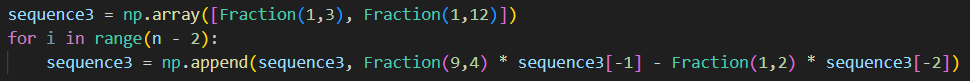
\includegraphics[width=1\linewidth]{fractions.png}
        \caption{Generowanie kolejnych elementów ciągu z użyciem klasy
        \texttt{Fraction} z biblioteki \texttt{fractions}.}
    \end{figure}

    \section{Przedstawienie wyników}
    \subsection{Zadanie 1.}
    \begin{figure}[H]
        \centering
        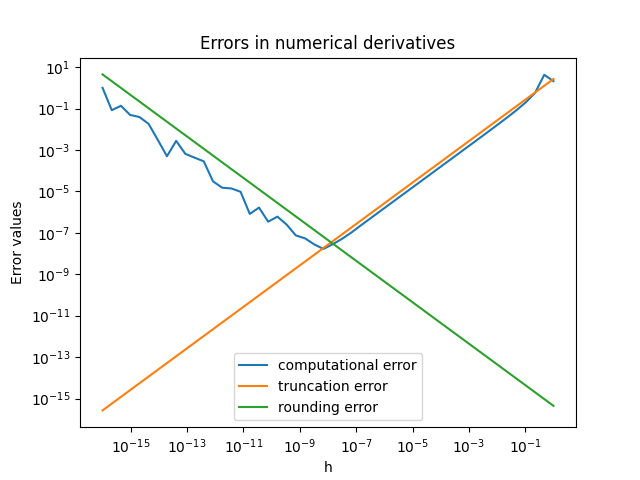
\includegraphics[width=0.8\linewidth]{Figure_1.png}
        \caption{Błędy dla wzoru różnic w przód.}
    \end{figure}
    \[
        h_{min}=6.866488450042998 \cdot 10^{-9}
    \]
    \[
        h_{min} \approx 2\sqrt{\frac{\epsilon_{mach}}{M}} \approx
        1.2902853526408846 \cdot 10^{-8}
    \]

    \begin{figure}[H]
        \centering
        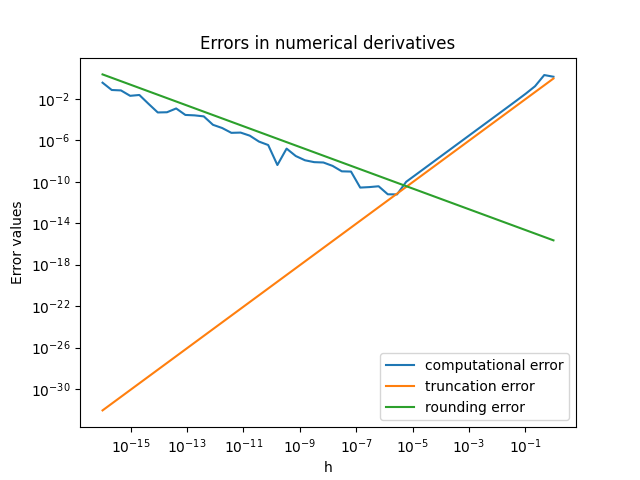
\includegraphics[width=0.8\linewidth]{Figure_2.png}
        \caption{Błędy dla wzoru różnic centralnych.}
    \end{figure}
    \[
        h_{min}=2.811768697974231 \cdot 10^{-6}
    \]
    \[
        h_{min} \approx \sqrt[3]{\frac{3\epsilon_{mach}}{M}} \approx
        2.2732741568390613 \cdot 10^{-6}
    \]

    \subsection{Zadanie 2.}
    \begin{figure}[H]
        \centering
        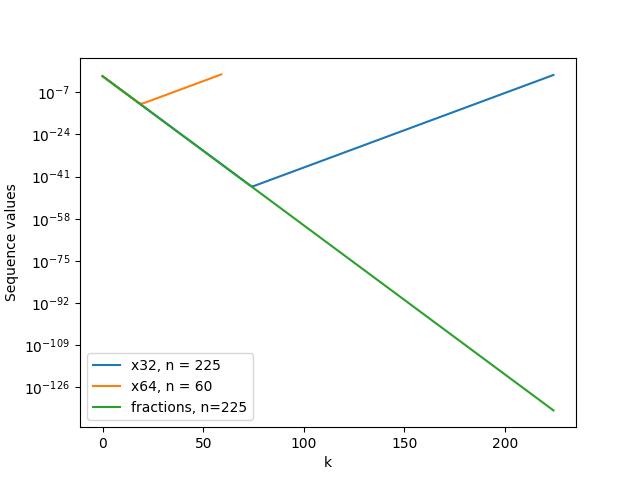
\includegraphics[width=0.8\linewidth]{seq.png}
        \caption{Wartości ciągu generowane różnymi metodami.}
    \end{figure}
    \begin{figure}[H]
        \centering
        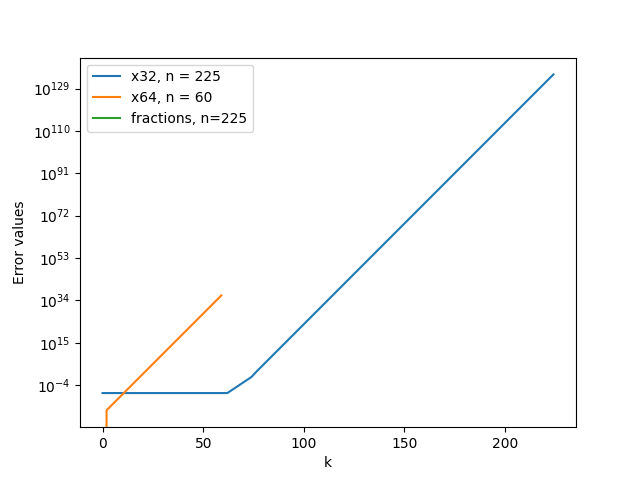
\includegraphics[width=0.8\linewidth]{seq_error.png}
        \caption{Wartości błędu względnego generowane różnymi metodami.}
    \end{figure}
    \subsection*{}
    W przypadku użycia biblioteki \texttt{fractions} wartość błędu dla $n=225$
    jest stale równa $0$.
    
    \section{Wnioski}
    \subsection{Zadanie 1.}
    W obliczeniach z użyciem wzoru różnic centralnych wartości błędu
    obliczeniowego mają znacznie większy zakres górny i dolny. Najmniejsza
    wartość błędu obliczeniowego przyjmowana jest dla
    $h_{min} \approx 6.87 \cdot 10^{-9}$ w przypadku wzoru różnic w przód, a dla
    wzoru różnic centralnych $h_{min} \approx 2.81 \cdot 10^{-6}$. Jest ono
    zbliżone do prawdziwego. Dla mniejszych $h$ niż $h_{min}$ wartość błędu
    obliczeniowego zaczyna rosnąć. Może to być spowodowane zbyt małymi
    wartościami $h$ wykraczającymi poza precyzję obliczeń.

    \subsection{Zadanie 2.}
    Kolejne wartości ciągu, wyznaczane z użyciem pojedynczej precyzji, znacznie
    szybciej zaczynają rosnąć, niż w przypadku podwójnej precyzji. Ze wzoru
    jawnego ciągu wiemy, że jest on malejący. Zmiana monotoniczności wynika
    prawdopodobnie z przekroczenia dokładności liczby zmiennoprzecinkowej
    w języku Python. Użycie klasy \texttt{Fraction} z biblioteki \texttt{fractions}
    pozwala na dokładne wyznaczanie wartości ciągu dla $n=225$, ponieważ
    przechowujemy osobno licznik i mianownik, dzięki czemu możemy uniknąć
    utraty precyzji. \\
    Z powyższego wynika błąd względny, który dla obliczeń pojedynczej precyzji
    znacznie szybciej zaczyna rosnąć niż w przypadku obliczeń podwójnej precyzji.
    Obliczenia z użyciem biblioteki \texttt{fractions} pozwalają na utrzymanie
    błędu względnego na poziomie $0$.

    \subsection{Podsumowanie}
    Dzięki wykonanym obliczeniom można zauważyć, że arytmetyka zmiennoprzecinkowa
    w komputerze nie jest idealna. Wykonując obliczenia numeryczne należy pamiętać
    o ograniczeniach sprzętowych komputerów, ponieważ nierozważne wykonywanie
    obliczeń może prowadzić do poważnych błędów.

    \section{Bibliografia}
    \url{http://heath.cs.illinois.edu/scicomp/notes/cs450_chapt01.pdf} \\
    \url{https://pl.wikipedia.org/wiki/Liczba_zmiennoprzecinkowa} \\
    \url{https://pl.wikipedia.org/wiki/B%C5%82%C4%85d_przybli%C5%BCenia}

\end{document}
